\documentclass[sigconf]{acmart}

\usepackage{algorithmic}
\usepackage{algorithm}
\usepackage{hyperref}
\usepackage{caption}
\usepackage{subcaption}

\begin{document}

\title{Lab 4 Exercise - Fun with MLPs \& MNIST}
\author{Luke McClure}
\email{29573904}

\maketitle

\section{Exercise 1}
\subsection{Wide MLPs on MNIST}

To conduct this experiment, a range of single layered MLP's were trained with hidden layer's sized $2^n$ from $n = 1$ until $n = 16$, for a max hidden layer size of 65,536 neurons.
The Adam optimiser was used to train at a default learning rate over 25 epochs.

With 60,000 samples in the MNIST training dataset, with anything over $2^{7} = 128$ nodes in the hidden layer, there will be 101,770 learnable parameters in the network, more than enough to start to overfit to the dataset.

\begin{table}
    \begin{tabular}{|c c c c c|}
        n & Hidden Layer Size & Parameters & Train Accuracy & Test Acc \\
        \hline
        1 & 2 & 1,600 & 0.403 & 0.407 \\        
        2 & 4 & 3,190 & 0.691 & 0.686 \\
        3 & 8 & 6,370 & 0.864 & 0.861 \\
        4 & 16 & 12,730 & 0.929 & 0.923 \\
        5 & 32 & 25,450 & 0.965 & 0.957 \\
        6 & 64 & 50,890 & 0.987 & 0.969\\
        7 & 128 & 101,770 & 0.998 & 0.975\\
        8 & 256 & 203,530 & 1.000 & 0.980\\
        9 & 512 & 407,050 & 1.000 & 0.982\\
        10 & 1024 & 814,090 & 1.000 & 0.983\\
        11 & 2,048 & 1,628,170 & 1.000 & 0.985\\    
        12 & 4,096 & 3,256,330 & 1.000 & 0.987\\
        13 & 8,192 & 6,512,650 & 0.999 & 0.985\\
        14 & 16,384 & 13,025,290 & 0.996 & 0.979\\
        15 & 32,768 & 26,050,570 & 0.997 & 0.979\\
        16 & 65,536 & 52,101,130 & 0.998 & 0.980\\
    \end{tabular}
\end{table}

Investigating the training curves shown in \autoref{fig:all}, it is clear to see small networks with 1-2 hidden nodes struggling to learn with maximum accuracies at 0.4 and 0.6 respectively.
For any MLP above 32 hidden units the training accuracy and loss quickly converge to close to perfect scores over the training data.

\begin{figure}
    \centering
    \begin{subfigure}{.25\textwidth}
        \centering
        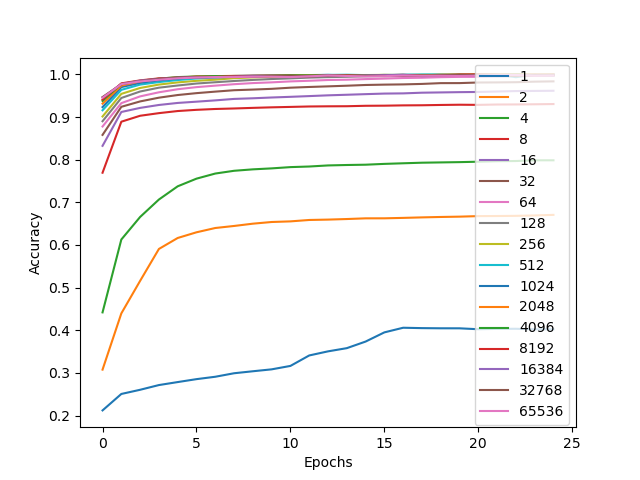
\includegraphics[width=\linewidth]{../allacc.png}
        \caption{Accuracy}
        \label{fig:allacc}
    \end{subfigure}%
    \begin{subfigure}{.25\textwidth}
        \centering
        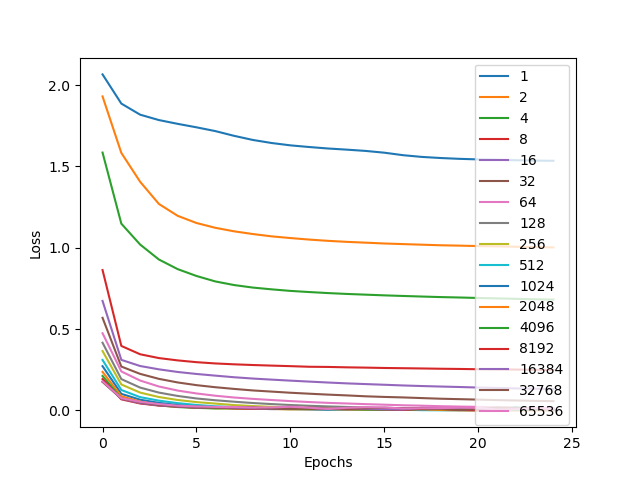
\includegraphics[width=\linewidth]{../allLosses.png}
        \caption{Loss}
        \label{fig:allloss}
    \end{subfigure}
    \caption{Showing training accuracy and loss across all models}
    \label{fig:all}
\end{figure}


With the scale of data presented, it is much easier to present the loss and accuracy compared to hidden unit on a logarithmic scale.
The data shown in \autoref{fig:log} show how the the final training and testing accuracy stays tightly bound until $2^{3}$, at which point the training accuracy started to overtake the testing accuracy.
This could be a sign of the network starting to overfit to the data, but I find it hard to claim that the network has failed to generalise to the dataset as the accuracy is still above 0.95.

The loss curves per hidden unit shown in \autoref{fig:losslog} are an interesting addition to this data. The loss shown in these curves start to level off past $2^{3}$, indicating the network is not able to utilise the extra width past this point.
\begin{figure}
    \centering
    \begin{subfigure}{.25\textwidth}
      \centering
      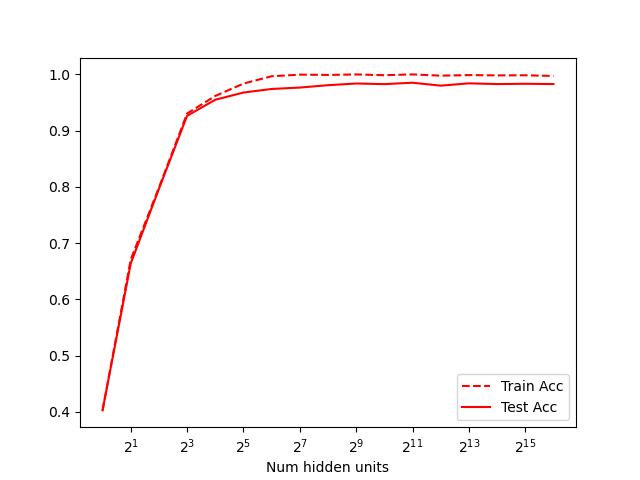
\includegraphics[width=\linewidth]{../acclog.png}
      \caption{Accuracy}
      \label{fig:acclog}
    \end{subfigure}%
    \begin{subfigure}{.25\textwidth}
      \centering
      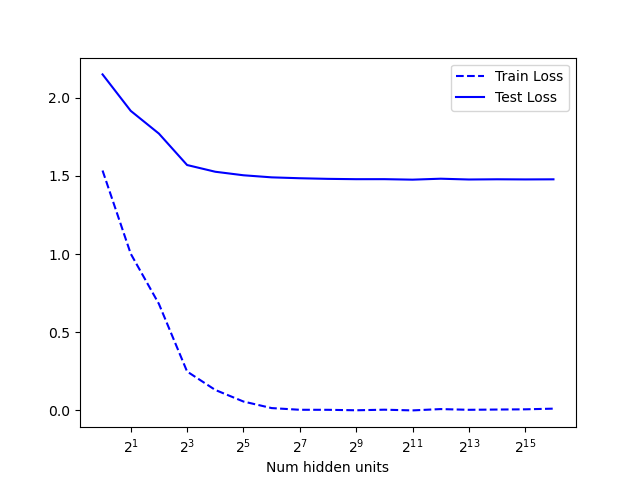
\includegraphics[width=\linewidth]{../losslog.png}
      \caption{Loss}
      \label{fig:losslog}
    \end{subfigure}
    \caption{Showing accuracy and loss on a log scale of hidden nodes}
    \label{fig:log}
\end{figure}

Over the course of this investigation I found it very hard to find clear signs of the models overfitting, even with hidden layers as wide as 65,536 neurons, 
the MNIST dataset may be a reasonably easily linearly seperable problem which would make it hard to overfit to.
\end{document}
\endinput